\chapter{Methodology}\label{methodik}
This chapter explores how GPUs convey information using a shared memory and defines what communication means in the context of this work. Using this definition, the analysis space is described and explored.
\section{GPU Shared Memory Communication}
Other than the explicit communication routines of MPI like send and receive, GPUs convey information implicitly via the global memory on the device. 
The CUDA execution model and the given guarantees can be mapped to the Bulk-Synchronous-Parallel (BSP) bridging model, explained in \ref{sec:bsp}.
\begin{itemize}
	\item \textbf{Computation} is a kernel executed on the GPU. The local components in the model are represented by CTAs on a GPU. Although BSP allows shared memory interactions, CUDA does not, therefore  each CTA is processing it's own workload without the ability to directly interact with other CTAs. 
	\item \textbf{Communication} in this step data generated in the computation step is placed in a location where it can be accessed by a component using the data in a following superstep. For GPUs this location is 
	global memory, because it is modifiable by a kernel during execution and it's modifications persist beyond kernel completion boundaries. In other words, global memory is a memory area allowing visible side-effects
	of a kernel execution.
	\item \textbf{Synchronization} on the GPU happens implicitly by the kernel completion boundary. It guarantees visibility of all global memory operations by the kernel. This implies that follow-up supersteps can see the memory modifications. Just as the barrier in BSP makes sure the communication step
	has been completed by all processors. Partial synchronization is only possble if kernels are members of different streams.
\end{itemize} 
 Not all of the side-effects mentioned above however, can be classified as communication. In the context of this work, communication is data that is written to global memory by one thread and read by another. The CUDA consistency model allows reliable communication only across kernel completion boundaries. We only consider elements that are communicated reliably.

\begin{figure}[t]
	\centering
	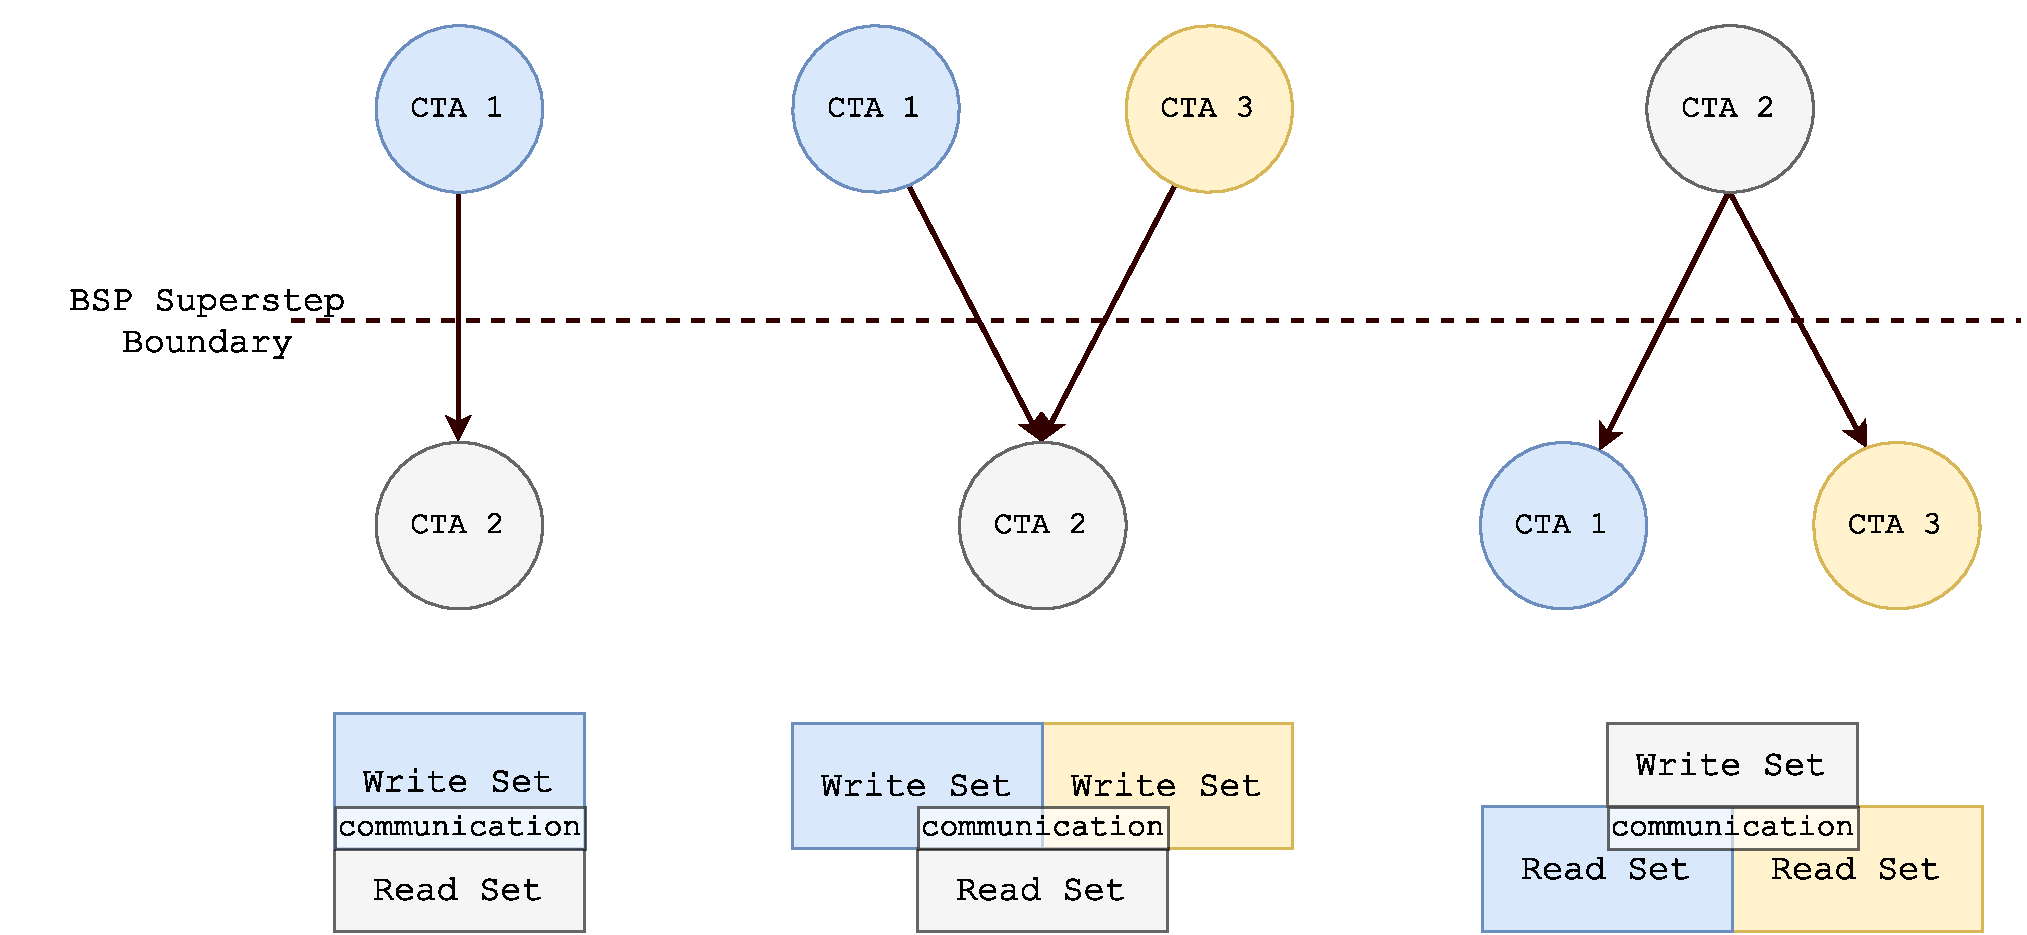
\includegraphics[width=\textwidth]{gpu-comm}
	\caption[CTA Communication]{Communication of CTAs across a BSP superstep boundary, and how this corresponds to read and write sets 
	of sinks and sources. Edges are logical representations of communication, which is actually the overlap of write and read addresses in different BSP supersteps. Different colors represent different sink/source entities.}
	\label{gpu-comm}
\end{figure} 
To exemplify the definition above, figure \ref{gpu-comm} shows how communication between CTAs across a 
BSP superstep boundary translates to overlaps of write- and read-sets. The nodes above the superstep boundary are data sources, the nodes below sinks. The accumulated edge-weight is the size of the 
overlapping area in the write- and read-sets. The left-most graph is a simple point-to-point connection, the middle one resembles a gather collective and the right-most graph can be a scatter or multicast, depending on the overlap. More on collectives in \ref{collectives}.
This representation works for all levels of granularity in the hierarchy of the GPU execution model, from a single thread to an application using multiple kernels and streams.

\section{Analysis Space Exploration}

The analysis space for this work can be separated into spatial and temporal dimensions. The spatial dimension includes the layered hierarchy of threads, CTAs and Kernels. Each hierarchy layer is the superset of the underlying layers. For example, the total data volume written by a kernel is the sum of all its CTA's writes. 
Granularity determines how detailed the spatial dimension is analysed.
The coarsest granularity would be a complete application with multiple kernels and iterations, and the finest a single thread. For this work however, CTAs are used as the finest granularity. The spatial dimension can help characterize an application, but by itself cannot describe communication.

The temporal dimensions describes the series of executed BSP supersteps. Without this dimension, there is no communication to analyse, because by our definition, communication requires at least two subsequent supersteps.
Again, different granularity can be applied to the analysis. Granularity refines, as the term to describe the analysis in this dimension becomes more and more specific. The coarsest granularity ignores individual kernels and exclusively looks at the interaction between the existing supersteps. At finer granularities, the number of supersteps in the analysis may change, because only the interaction of two distinct kernels $k1$ and $k2$ across time $t$ is of interest.

\subsection{Analysis Methods}\label{methodik:methods}
Based on the dimensions and granularities, different tiers for the analysis can be defined.
\begin{enumerate}[I]
	\item Kernel behaviour across all supersteps
	\item Kernel interactions across two supersteps
	\item CTA interactions across two supersteps
\end{enumerate}
The analysis tries to avoid averaging and instead use aggregated values and relational metrics for comparison and analysis.


\subsection{Caveats}\label{collectives}
\begin{itemize}
	\item This work uses CTAs as the fundamental entities of communication source and sink, not threads.
	\item While MPI offers collective communication with clear definitions such as scatter, gather or multicast, the implicit memory communication of GPUs often can not be categorized as clearly. However the in- and out-degree of a communication entity might indicate tendencies towards a certain kind of collective.
	For the sake of the analysis, each collective communication ($\textrm{\{n:1\} \{1:n\} or \{n:n\}} $) can be viewed as a set of point-to-point communications, happening at the same time.
	\item  A kernel execution is a BSP superstep and is serialized with follow-up kernel iterations, or supersteps. Each stream is treated as
	an individual sequence of BSP supersteps during the execution. Stream interactions can be recreated in the follow-up analysis.
	\item Communication across BSP steps, honouring the guarantees CUDA's execution model gives, is not bound to any timing or ordering during the execution of a single compute kernel. Negative performance impacts by the instrumentation are therefore tolerated, 
	because in a well-written program the negative impact does not impede the correctness.
\end{itemize}